

All of the details in \cref{chapter:qhl} and \cref{chapter:qmla} are implemented in the \gls{qmla}
    software framework, a (mostly) Python codebase which underlies all of the 
    arguments, results and figures in this thesis. 
The codebase is designed to simplify the process of running \gls{qmla} or \gls{qhl}
    on novel systems.
In particular, the core \gls{qmla} algorithm can support a wide range of \glspl{es}, 
    allowing for the design of bespoke \glspl{es} to account for the specific requirements 
    of any given target system, \gls{q}. 
In this chapter we give an overview of the \gls{qmla} software, 
    implementation and instructions for its use. 
We do not introduce new mathematical, physical or algorithmic concepts, 
    so readers interested in applications of the techniques may prefer to skip to \cref{part:theoretical_study}.

\section{Implementation}
In this section we describe the technical details of the implementation of the 
    algorithm described in \cref{chapter:qmla}, as well as a number of relevant subroutines. 
These discussions aim first to familiarise readers with some fundamental programming conventions,
    and then describe how we can leverage those concepts to construct the \gls{qmla} infrastructure.

\subsection{Object oriented programming}
We first introduce the concepts of object-oriented programming, 
    and in particular \emph{inheritance} between objects, 
    since this will feature in later discussion about the implementation of \gls{qmla}
    and \glspl{es}. 
Python is a robust object-oriented language \cite{python-manual}, meaning that we can frame 
    concepts as \emph{objects}, permitting actions to be performed to/by them. 
In particular, objects in Python are formulated as \emph{classes}, 
    which can have associated \emph{attributes} and \emph{methods}. 
For example, we can encode the concept of a \ttt{Footballer} as a class,
    such that the player object holds attributes such as number of games played and goals scored in a season;
    the player objects also has methods which achieve specific calculations, 
    e.g. to summarise their record.
We can then utilise the \ttt{Footballer} class to store information about an \emph{individual} player, 
    by making an \emph{instance} of the class.
\par 

A fundamental concept in object-oriented programming is \emph{inheritance} between objects, 
    such that a \emph{child} object inherits properties of its \emph{parent}.
In general, a parent object can be thought of as an abstract concept, 
    which provides basic functionality and reasonable default properties,
    while a child object can incorporate specific requirements.
For example, an \ttt{Athlete} class can act as a parent to the \ttt{Footballer} class, 
    where the \ttt{Athlete} class holds core information such as date of birth. 
This allows for the \ttt{Athlete} class to be recycled as the \emph{base} class for other child classes
    which have the same underlying requirements, e.g \ttt{RubgyPlayer}. 
We list this example in \crefrange*{listing:athlete_class}{listing:footballer_class}. 

\begin{lstlisting}[
    label=listing:athlete_class,
    caption={Parent class, encoding the concept of an athlete. Programmed in Python.}
]
class Athlete():
    
    def __init__(
        self, 
        name, 
        birth_day, 
        birth_month, 
        birth_year, 
    ):
        # Use information given
        self.name = name
        self.date_of_birth = datetime.date(
            birth_year, birth_month, birth_day
        )
        
    def age(self, round_down=True):
        # Method to compute this athlete's age
        days_since_birth = ( 
            datetime.date.today() 
            - self.date_of_birth
        )
        age = days_since_birth.days / 365
        
        if round_down:
            age = int(age)
        
        return age
    
    def summary(self):
        # Method to summarise this athlete
        summary = "{name} is a {age}-year old athlete.".format(
            name = self.name, 
            age = self.age()
        )
        print(summary)
        
        
bob = Athlete(
    name='Bob',
    birth_day = 11,
    birth_month = 11, 
    birth_year = 1993, 
)
bob.summary()    
\end{lstlisting}

\begin{lstlisting}[
    label=listing:footballer_class,
    caption={Child class, encoding the concept of a footballer, which adopts the abstract representation of an athlete. 
        Programmed in Python.
    }
]
class Footballer(Athlete):
    def __init__(
        self, 
        footed,
        team, 
        size='medium',
        **kwargs
    ):
        # Pass arguments to the parent class
        super().__init__(**kwargs)
        
        # Use information given
        self.team = team
        self.footed = footed
        self.size = size
        
        # Default attributes
        self.goals_scored = 0 

    def summarise(self):
        # Overwrite parent's summarise method
        # with method specific to Footballers
        summary = ( 
            "{size} {player} plays for {team} and has scored {num_goals} goals.".format(
                size = self.size, 
                player = self.name, 
                team = self.team, 
                num_goals = self.goals_scored
            )
        )
        print(summary)
        
    def record_goals(self, num_new_goals):
        # Method to record that the Footballer 
        # has scored a number of new goals
        self.goals_scored += num_new_goals
        
# Make an instance of Footballer to represent an individual
mickey = Footballer(
    name = 'Mickey', 
    footed = 'left',
    team = 'QECDT-FC',
    birth_day = 11,
    birth_month = 11, 
    birth_year = 1993,
    size = 'Big'
)
# Call the methods on the instance
mickey.record_goals(num_new_goals = 10)
mickey.summarise()    
\end{lstlisting}

\section{Python framework}
\begin{figure}
    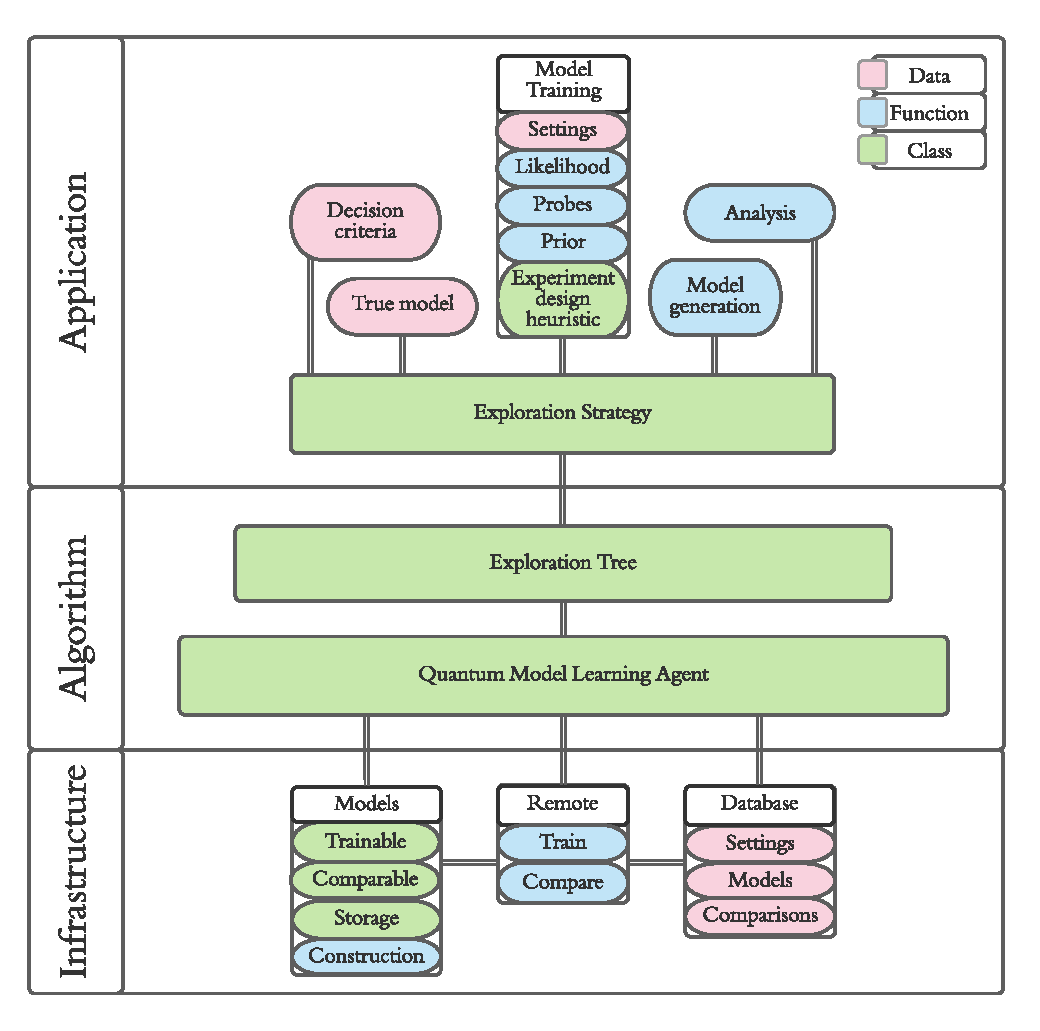
\includegraphics{algorithms/figures/software_overview.pdf}
    \caption[QMLA codebase overview]{
        Overview of important \emph{objects} in the \gls{qmla} framework.
        The objects' colour encodes its \emph{type}: 
            red objects are \emph{data/properties},
            blue are \emph{functions/methods} 
            and green are \emph{classes}. 
        Objects are grouped broady, with double lines showing communication channels between (groups of) objects. 
        \textbf{Infrastructure,} functions for the implementation of model training/comparisons on 
            a remote compute server, \cref{sec:infrastructure}.
        \textbf{Algorithm,} implementation of the iterative procedures and decision-making 
        laid out in \cref{chapter:qmla}. The algorithmic controls are detailed in \cref{sec:sw_algorithm}. 
        \textbf{Application,} inter-changeable data/functionality for the unique requirements 
        of a given target system, \cref{sec:application}. 
        Users wishing to customise \gls{qmla} must choose a valid implementation for each object in this segment
            but need not alter any of the underlying framework.
    }
    \label{fig:software_overview}
\end{figure}

A driving motivation for the development of \gls{qmla} is generality:
    we endevaour to make \gls{qmla} applicable to any target quantum system, \gls{q}.
We provide a framework, where users can tailor the inputs and methodology to their needs.
The main components of the framework are depicted in \cref{fig:software_overview}, 
    broadly grouping concepts as part of its \emph{infrastructure}, \emph{algorithm}
    or \emph{application}. 
In short, users need only specify the elements of the framework in the \emph{application} segment, 
    without concern for the underlying mechanics of \gls{qmla}.
In particular, users interface with the framework through the design of a bespoke \gls{es}, described next. 

\subsection{Application}\label{sec:application}
The application of \gls{qmla} refers to the choice of target system, \gls{q}, and how \gls{qmla} searches the 
     \gls{model space}  in attempt to uncover its model. 
As outlined in \cref{sec:exploration_strategies}, \glspl{es} play the role of 
    defining \gls{qmla}'s objectives, guiding the steps it takes, and designing the models to be tested. 
We facilitate the study of any system by providing a robust \ttt{ExplorationStrategy} base class,
    with all of the functionality expected of a generic \gls{es}, allowing users to inherit and build upon it. 
In particular, \glspl{es} allow users to specify the implementation of aspects listed in \cref{sec:exploration_strategies}, 
    as well as further details.
\par 


\subsubsection{Modular functionality}\label{sec:modular_functionality_sw}
The most crucial methods\footnotemark \ of the \gls{es} class are modular, 
    described in \cref{sec:modular_functionality},
    meaning that they can be directly replaced, provided the alternative method fulfils the same role. 
Our base \gls{es} class uses sensible defaults for this modular functionality, 
    but this flexible mechanism allows for adapting \gls{qmla} by choosing an approach for each 
    of the following subroutines. 
\footnotetext{
    The words \emph{method} and \emph{function} are mostly interchangeable, although methods are specifically associated with a class, 
    while functions are stand-alone.
}

\begin{easylist}[itemize]
    &  \Gls{likelihood} function. 
        As described in \cref{sec:likelihood}, the \gls{likelihood} is the means by which \gls{qhl} 
            trains candidate models.
        By default, \gls{qhl} calls a subroutine to compute \cref{eqn:likelihood}. 
        This can be replaced by any function which, given a \gls{hamiltonian}, evolution time and \gls{probe} state, 
        returns the \gls{likelihood}, according to the desired experiment for simulation.
        For example, in \cref{chapter:nv}, the data on which models are trained comes from experimental measurements, 
            so we replace the \gls{likelihood} function with a calculation corresponding to the experimental procedure. 
    & \Gls{probe} generation. 
        The training phase requires a set of probes against which to optimise individual models, 
            as examined in \cref{sec:probes}. 
        Users may wish to specify the design of such probes, for example to match experimental constraints 
        which restrict the realisible probes in the performance of the experiment. 
        Alternatively, it may be feasible to design probes which increase the information gained per experiment, 
        enabling faster learning. 
    & \Gls{edh}. The choice of \gls{edh} greatly influences how the training will perform, see \cref{sec:heuristic}. 
        We provide a base class implementing \gls{pgh}, as well as child classes for each of 
        the \glspl{edh} listed in \cref{sec:alt_heuristics}. 
    & Prior. The method of drawing the prior distribution can be replaced, for example, with 
        a method for constructing a uniform distribution on each parameter.
        A key input to the procedure is the initial knowledge the user has about the system, 
        which is encoded in the prior, for instance varying orders of magnitude of the viable terms.
\end{easylist}

Additionally, applications require a series of settings for the model training phase, 
    such as the \glspl{hyperparameter} required by the resampling algorithm, \cite{liu2001combined}, 
    as well as detailing the \gls{true model}, $\ho$, in the case where \gls{q} is simulated.
We can also direct \gls{qmla} to perform \gls{es}-specific analyses to examine its internal performance, 
    although this is generally required during development/testing, and less useful thereafter. 

\subsection{Algorithm}\label{sec:sw_algorithm}
The algorithm layer of \cref{fig:software_overview} implements the core steps of \gls{qmla},
    as shown in \cref{fig:qmla_overview}, by running a set of \acrfullpl{et}, 
    each of which communicate with a unique \gls{es}. 
The core \gls{qmla} class manages the database of models and their comparisons,
    and decides how to react at certain stages, by consulting the decision criteria set by the \gls{es}. 
\par 

% \subsubsection{Parallel implementiation}\label{sec:parallel}
\begin{figure}
    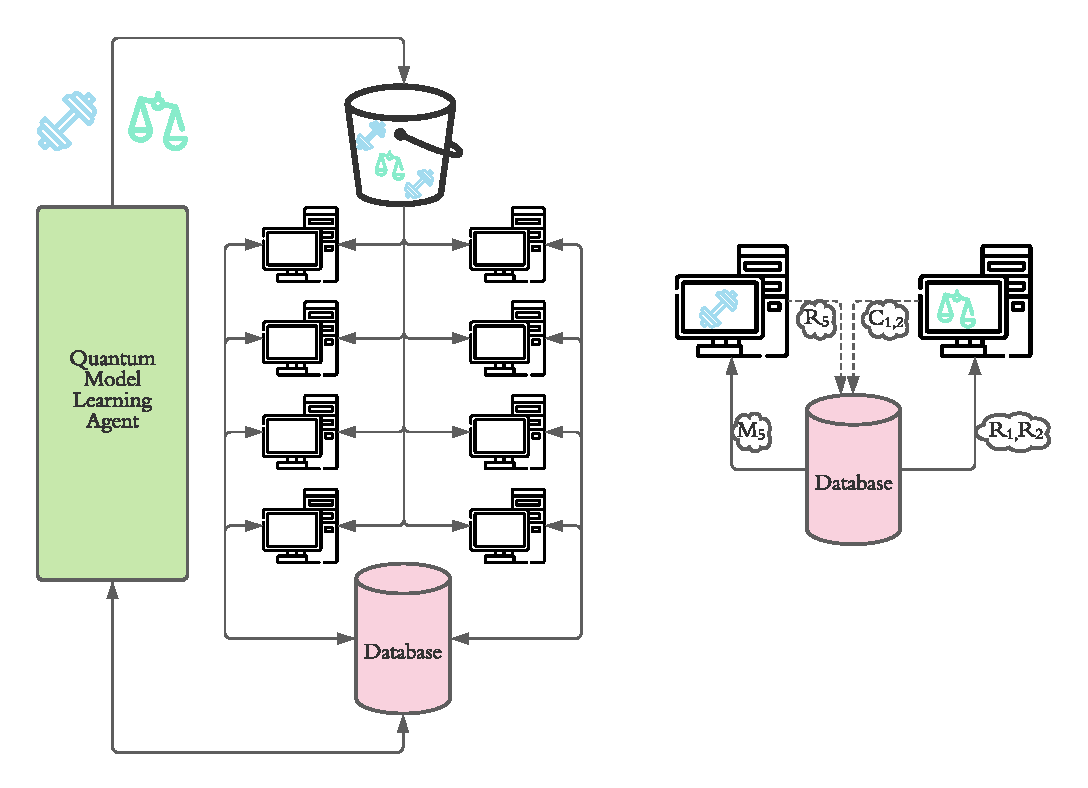
\includegraphics{algorithms/figures/parallel_architecture.pdf}
    \caption[Parallel architecture for QMLA]{
        Parallel architecture for \acrfull{qmla}.
        \textbf{Left,} \gls{qmla} generates tasks 
            -- either to train (blue dumbbells) or compare (green scales) models -- 
            and places them in a task queue. 
        Worker processes (depicted as computers) retrieve those tasks and compute them in parallel, 
            and interact with a database. 
        \textbf{Right,} Distributed tasks occuring in parallel, with each process communicating with the database. 
        The left-hand process assumes the task of training the model with ID 5, $\hat{H}_5$:
            it first queries the database for a packet of core information, $M_5$, 
            which informs the model training procedure, for example the terms and parameters 
            of $\hat{H}_5$. 
        After training, it sends a packet, $R_5$, summarising the result of $\hat{H}_5$'s training. 
        The right-hand process compares two models with IDs 1 and 2, by first retrievng the results packets
            $R_1, R_2$, then storing the comparison $C_{1,2}$ on the database. 
    }
    \label{fig:parallel}
\end{figure}

The implementation of \gls{qmla} seeks to separate the organisation of the  \gls{model search}  from the 
    cumbersome calculations which enable the search. 
We can offload those calculations to a compute cluster (server) to run \emph{in parallel},
    allowing for significant speedup of the entire \gls{qmla} procedure, 
    limited by Amdahl's law. 
Amdahl's law stipulates that the \emph{speedup} available to any program due to parallelisation 
    is limited by the portion of the program which is inherently parallelisable, versus inherently serial \cite{hill2008amdahl}.
In \gls{qmla}, all the model training and model comparison subroutines can be run in parallel, 
    while only the administrative steps of the core \gls{qmla} algorithm are inherently serial, 
    so \gls{qmla} can benefit greatly from parallelism.
\par

While there are a number of strategies for parallelising code over a cluster of individual \emph{processes}\footnote{Each process is a single \acrshort{cpu}}, 
    we use the \emph{master-worker} strategy, where one process acts as the \emph{master}, 
    determining which calculations are required at any given moment, 
    then brokering self-contained \emph{tasks} to \emph{workers}, 
    which blindly solve a small problem, without knowledge of the wider context or algorithm \cite{hockney2019parallel}.
The mapping here is trivial: the master of our algorithm is \gls{qmla}, 
    while workers can be used for the tasks of training and comparing models. 
\gls{qmla} distributes tasks to worker processes in a server, 
    i.e. we assume that \gls{qmla} is run on a machine with $N_c$ available parallel \emph{processes}\footnotemark. 
One process is designated for the \gls{qmla} class alone,
    e.g. for the ranking of models and determination of the next models to tests, 
    while the remaining $N_c - 1$ processes lay dormant until \gls{qmla} requests that they perform a task. 
The role of \gls{qmla} is to collate the outcome of those calculations in conjunction with the set of \glspl{et}, 
    until each \gls{et} is deemed complete, and then to consolidate the set of 
    \gls{et} champions, ultimately setting the global champion, $\hp$. 
Thereafter it can perform some analysis; see \cref{sec:qmla_outputs} for further details. 

\footnotetext{Note when running in \emph{serial} (e.g. running locally on a personal machine), it is valid to simply set $N_c=1$.}
\par 
\gls{qmla} and all workers have shared access to a database, through which they communciate data pertaining to individual tasks \cite{redis}. 
We use a simple \emph{task queue} for the distribution of jobs: 
    \gls{qmla} adds tasks to the queue and any available worker can take the next job and compute it \cite{redis_queue}.
The queue can be accessed by only one thread at a time, to ensure tasks are not duplicated. 
There are two types of task for workers:
\begin{easylist}
    & to train a candidate model, $\hi$:
        the worker first requests some essential information about the model from the database, 
        e.g. the name, terms and prior associated with the model, packaged in $M_i$;
        following completion, the worker compresses the result, $R_i$, and sends it to the database for storage. 
    & to compare two models, $\hi, \hj$: 
        the worker retrieves $R_i, R_j$ from the database, performs the calculation, 
        and returns the compressed outcome of the comparison, $C_{ij}$, to the database. 
\end{easylist}
The \gls{qmla} class copies the compressed results packets $R_i$ and $C_{ij}$,
    in order to account for the results in its decision-making. 
It is worth noting that tasks are completely independent, so some worker processes
    may compute comparisons while others train models simultaneously, 
    although the comparison between $\hi, \hj$ can not begin until both $R_i, R_j$ are available. 
To ensure tasks are not launched in advance of their dependencies, we enforce a \emph{blocking} protocol, 
    whereby new batches of jobs are not released until the master receives all the results of jobs on which the new tasks depend:
    \gls{qmla} simply waits until all models on a given branch have been trained before queueing comparisons 
    on that branch.
\par

Models are assigned a unique ID upon creation,
    and are uniquely described by their name, represented as a string in the \gls{qmla} class, 
    such that newly proposed models can be checked against the set of previously considered models 
    before being added to the database. 
\gls{qmla} can hence check whether a proposed model, $\hi$, has already been trained, 
    in which case it does not resubmit the model, but instead relies on the existing result, $R_i$. 
Likewise \gls{qmla} can check for the presence of any comparison result, $C_{ij}$, 
    before submitting the comparison as a new task, 
    ensuring we do not duplicate expensive calculation. 
We depict the structure of this parallel architecture, and the master-worker strategy, in \cref{fig:parallel}.

\subsection{Infrastructure}\label{sec:infrastructure}
The infrastructure enabling the distribution of \gls{qmla}'s tasks across 
    a set of worker processes can be summarised as:
\begin{easylist}
    & a set of classes representing the objects on which we must perform expensive calculations;
    & functions to launch those calculations independently of any other calculation;
    & a database which can be accessed by all workers as well as the \gls{qmla} master class.
\end{easylist}
\par 

We need a series of distinct classes to represent models, for use in each stage of \gls{qmla}: 
    a \emph{trainable} class is used for the parameter optimisation, 
    while \emph{comparable} classes are used for computing \glspl{bf}.
Crucially, this separation allows us to perform data-heavy calculations independently, 
    e.g. on a remote process within a compute cluster, 
    and discard the class instance used for the calculation and the large amount of data it generates, 
    while only the relatively small \emph{storage} class is retained by \gls{qmla} for later use. 

\par 
The tasks which actually implement the calculations (\cref{sec:sw_algorithm}) are captured by standalone \emph{remote} functions. 
These functions receive instructions such as \ttt{train model 10}; 
    they then contact the database for the set of shared settings, 
    such as \gls{nexp}, \gls{nprt} and the set of probes, 
    before performing the task, and then send the compressed result, $R_{10}$, to the database for storage.  
To achieve this separation between calculation and analysis, we use a redis database \cite{redis},
    which holds the core implementation settings, e.g. \gls{nexp}, \gls{nprt} and the set of probes to train upon, 
    as well as the compressed summaries of the outcomes of tasks.

\section{Usage}\label{sec:usage}

Several aspects of \gls{qmla} are \emph{probabilistic}.
Firstly, the Bayesian updates within model training -- i.e. \gls{qhl} --
    relies on \glspl{likelihood} which 
    implicitly depend on the measurement datum of a quantum system.
In the case where the projective measurement finds \gls{q} in a less-likely eigenstate, 
    i.e. one with lower probability immediately prior to measurement, 
    the \glspl{likelihood}  will indicate poor outcomes from good hypotheses, 
    resulting in misguided posterior distributions. 
It is thus \emph{possible} that the parameter learning will converge on incorrect values,
    or not converge at all even given ample resources. 
Moreover, the model design subroutine is not gauranteed to exploit the aspects of favoured models which are 
    actually informative, e.g. given a favoured model with four correct terms and two incorrect terms, 
    the model generator may opt to build upon the incorrect terms, in the common situation where it can not distinguish between 
    helpful and misleading constituent terms.
\par 

Overall then, 
    it is pertinent to run the entire \gls{qmla} algorithm repeatedly and gather statistics about its performance and outcomes, 
    rather than making definitive claims about \gls{q} based on a single implementation.
We say that a single implementation of \gls{qmla} is an \emph{\gls{instance}},
    and $N_r$ \glspl{instance} are grouped in a \emph{\gls{run}}.
\Glspl{instance} can be realised in parallel, 
    each relying on the master-worker parallel structure laid out above. 
We are primarily concerned with the performance of the \gls{run} 
    instead of any individual instance. 
For example,
    for each model, $\hi$, in the \gls{model space}, we can interpret its \emph{ \gls{win rate} } 
    -- the fraction of instances for which \gls{qmla} finds $\hp=\hi$ -- 
    as evidence for that $\ho=\hi$.
For the sake of evaluating \gls{qmla} itself, as in \cref{part:theoretical_study}, 
    we can use the  \gls{win rate}  of $\ho$ as indication of the overall \emph{\gls{success rate}}, 
    i.e. the fraction of \glspl{instance} within a run where \gls{qmla} identifies precisely $\hp = \ho$. 
Note, however, that neither the  \gls{win rate}  nor \gls{success rate} are singularly informative 
    of \gls{qmla}'s performance: in some cases, we can deem \gls{qmla} successful even if it does not 
    identify $\ho$ exactly, e.g. if it finds the majority of terms present in $\termset_0$ from a large space, 
    i.e. a high $\fs$, see \cref{sec:f_score}. 
\par 

The \gls{qmla} codebase is available at \cite{flynn2021QMLA},  
    with complete documentation including a tutorial at \cite{qmla_docs}. 
We show how to design a custom \gls{es} and incorporate it within \gls{qmla}, 
    and deploy the computation on a cluster in \cref{apdx:software_eg}.

\subsection{Outputs and analysis}\label{sec:qmla_outputs}
When a \gls{run} is launched, \gls{qmla} generates a \emph{\gls{results directory}} unique to that \gls{run}, 
    identified by the time and date of its launch,
    in which all the pertinent information for that \gls{run}, including raw data and figures, are stored. 
It includes an \ttt{analyse.sh} script to generate analysis after all \glspl{instance} have completed\footnotemark. 
\gls{qmla} provides a large amount of analytics to assess the performance of the protocol. 
These range from \emph{big picture} perspectives such as the  \gls{win rate}  across the entire \gls{run}, 
    to focusing on internal metrics for training individual models.
Some of these analyses are generated by default, while others are optional depending on the 
    level of detail the user requires. 
A number of sub-directories are produced in the \gls{results directory}, 
    each containing data/figures from a different view of the \gls{run};
    these are listed in \cref{apdx:figure_repoduction}.
Results are categorised across the levels of the framework, the most important of which are:

\footnotetext{
    Note this script is not run automatically since, on remote servers, \glspl{instance} finish independently without any central process
    noticing. Therefore this script must be run by the user when the run is complete.
}
\begin{description}
    \item[\Gls{run}] \ 
    
    Results across a number of instances.
    \begin{easylist}
        && \Glspl{win rate} for all models which are found as \gls{champion model} at least once.
        && Average dynamics reproduced by \glspl{champion model}.
    \end{easylist}
    
    \item[\Gls{instance}] \ 
    
    Performance of a single \gls{instance}.
    \begin{easylist}
        && Models generated and the branches on which they reside.
    \end{easylist}

    \item[\Gls{model}] \  
    
    Individual model performance within an instance.
    \begin{easylist}
        && Parameter estimation through \gls{qhl}.
    \end{easylist}

    \item[Pairwise Comparisons] \ 
    
    Direct comparison of models’ performance.
    \begin{easylist}
        && Dynamics of both candidates (with respect to a single basis).
    \end{easylist}

    \item[\Acrlong{es}] \ 
    
    Analysis specific to the \gls{es}.
    \begin{easylist}
        && For example, model generation metrics.
    \end{easylist}
\end{description}
\par 


Most plots used in this thesis are generated directly by the \gls{qmla} framework\footnotemark; 
    complete details for reproducing each figure are listed in \cref{table:figure_reproduction}, 
    with further details for navigating \gls{qmla}'s outputs in \cref{apdx:figure_repoduction}. 
Examples of some of the available analyses, as well as a demonstration for customising the \gls{qmla} software
    is given in \cref{apdx:software_eg}.

\footnotetext{
    Figures presented in this thesis are minor modifications of figures available for automatic analysis in \gls{qmla}.
}
